\documentclass[12pt]{article}
% Load packages
\usepackage{url}  % Formatting web addresses
\usepackage{ifthen}  % Conditional
\usepackage{multicol}   %Columns
\usepackage[utf8]{inputenc} %unicode support
\usepackage{amsmath}
\usepackage{amssymb}
\usepackage{epsfig}
\usepackage{epstopdf}
\usepackage{graphicx}
\usepackage[margin=0.1pt,font=footnotesize,labelfont=bf]{caption}
\usepackage{setspace}
%\usepackage{longtable}
\usepackage{colortbl}
%\usepackage{palatino,lettrine}
%\usepackage{times}
%\usepackage[applemac]{inputenc} %applemac support if unicode package fails
%\usepackage[latin1]{inputenc} %UNIX support if unicode package fails
\usepackage[wide]{sidecap}
%\usepackage[authoryear,round,comma,sort&compress]{natbib}
\usepackage[square,sort,comma,numbers]{natbib}
%\usepackage[authoryear,round]{natbib}
\usepackage{supertabular}
\usepackage{simplemargins}
\usepackage{comment}
\usepackage{lineno}

\urlstyle{rm}

%\textwidth = 6.50 in
%\textheight = 9.5 in
%\oddsidemargin =  0.0 in
%\evensidemargin = 0.0 in
%\topmargin = -0.50 in
%\headheight = 0.0 in
%\headsep = 0.25 in
%\parskip = 0.15in
%\linespread{1.75}
\doublespace

%\usepackage{geometry}
\usepackage{fullpage}

%\bibliographystyle{plain}
\bibliographystyle{msb}

\makeatletter
\renewcommand\subsection{\@startsection
	{subsection}{2}{0mm}
	{-0.05in}
	{-0.5\baselineskip}
	{\normalfont\normalsize\bfseries}}
\renewcommand\subsubsection{\@startsection
	{subsubsection}{2}{0mm}
	{-0.05in}
	{-0.5\baselineskip}
	{\normalfont\normalsize\itshape}}
\renewcommand\section{\@startsection
	{subsection}{2}{0mm}
	{-0.2in}
	{0.05\baselineskip}
	{\normalfont\large\bfseries}}
\renewcommand\paragraph{\@startsection
	{paragraph}{2}{0mm}
	{-0.05in}
	{-0.5\baselineskip}
	{\normalfont\normalsize\itshape}}
\makeatother

%Review style settings
%\newenvironment{bmcformat}{\begin{raggedright}\baselineskip20pt\sloppy\setboolean{publ}{false}}{\end{raggedright}\baselineskip20pt\sloppy}

%Publication style settings

% Single space'd bib -
\setlength\bibsep{0pt}

\renewcommand{\rmdefault}{phv}\renewcommand{\sfdefault}{phv}

% Change the number format in the ref list -
\renewcommand{\bibnumfmt}[1]{#1.}

% Change Figure to Fig.
\renewcommand{\figurename}{Fig.}

% Begin ...
\begin{document}
\begin{titlepage}
{\par\centering\textbf{\Large Physical and Logical Models of Signal Transduction Processes in Cancer}}
\vspace{0.05in}
{\par \centering \large{ Katharine V. Rogers, Holly A. Jensen,
and Jeffrey D. Varner$^{*}$}}
\vspace{0.10in}
{\par \centering \large{School of Chemical and Biomolecular Engineering}}
{\par \centering \large{Cornell University, Ithaca NY 14853}}
\vspace{0.1in}
{\par \centering \textbf{Running Title:}~Physical and Logical Models of Signal Transduction Processes in Cancer}
\vspace{0.1in}
{\par \centering \textbf{To be submitted:}~\emph{}}
\vspace{0.5in}
{\par \centering $^{*}$Corresponding author current address:}
{\par \centering Jeffrey D. Varner,}
{\par \centering Professor, School of Chemical Engineering,}
{\par \centering 1158 Forney Hall, Purdue University, West Lafayette IN, 46907}
{\par \centering Email: jdvarner@purdue.edu}
{\par \centering Phone: (765) 496 - 0544}
\end{titlepage}
\date{}
\thispagestyle{empty}
\pagebreak
%%%%%%%%%%%%%%%%%%%%%%%%%%%%%%%%%%%%%%%%%%%%%%%%%%%%%%%%%%%%%%%%%%%%%%%%%%%%%%%%%%%%%%%%%%%%%%%%%%%%%%%%%%%
%%%%%%%%%%%%%%%%%%%%%%%%%%%%%%%%%%%%%%%%%%%%%%%%%%%%%%%%%%%%%%%%%%%%%%%%%%%%%%%%%%%%%%%%%%%%%%%%%%%%%%%%%%%
\section*{Abstract}


\vspace{0.5in}
{\noindent \textbf{Keywords:}~ cancer, mathematical modeling}

\pagebreak

\setcounter{page}{1}

\linenumbers

\section*{Introduction}

Cancer, once considered a monolithic disease, is a vast repertoire of diseases divided into carcinomas (epithelial-originating cancers), sarcomas (connective tissue cancers), leukemias (blood cancers), lymphomas, myelomas, and mixed types like teratocarcinoma. 
All these diseases exhibit the \textquotedblleft Hallmarks of Cancer\textquotedblright $\:$ as described by Hanahan and Weinburg in 2000 \cite{Hanahan2000}. 
These characteristics are (1) sustained proliferative signaling, (2) insensitivity to or evasion of growth-suppressive signals, (3) resistance to or evasion of apoptosis, (4) limitless renewal potential, (5) promotion of angiogenesis and (6) tissue invasion and metastasis. In a more recent review, to this list Hanahan and Weinburg added (7) altered metabolic signaling, and (8) resistance to immune destruction and resulting inflammation \cite{Hanahan2011}. 
These proposed hallmarks have in fact been criticized: it was pointed out that 5 of the original 6 (excluding ability to metastasize) are in fact characteristics of benign tumors as well \cite{Lazebnik2010}. 
Nonetheless, a general consensus exists that cancers do exhibit the above listed attributes, which can parsimoniously be described as notably harmful uncontrolled cell proliferation. 
Cancer can unfortunately arise in essentially any tissue type, resulting in \textquotedblleft hundreds of different cancers\textquotedblright $\:$ \cite{CancerGovClasses}.  

Cancer treatments have progressed over the years from surgery and chemotherapy to targeted therapies. 
Currently, there are a multitude of small molecule inhibitors on the market, including tyrosine kinase inhibitors, growth factor receptor inhibitors, mTOR inhibitors, and angiogenesis inhibitors. In addition, cancer vaccines are another up-and-coming therapy; Sipuleucel-T (Provenge) is an approved autologous vaccine for castration resistant prostate cancer \cite{Vanneman2012}.
%; the result is that T cell activity is simulated against the protein PAP (prostatic acid phosphatase) which is expressed by prostate cancer cells  
However, targeted therapies are proving less promising than previously anticipated. 
Of all anticancer agents tested in the preclinical setting, only 5\% are successfully licensed after making it to Phase III clinical testing \cite{Hutchinson2011}. 
This low success rate is mainly due to poor candidate selection in the preclinical arena, which arises from shortcomings on how cancer therapies are pursued. 
Individual cell lines do not represent whole cancers; mouse xenografts do not reflect the human case; treatments are tested as monotherapeutics rather than combination therapies. 
Bevacizumab (Avastin) was a previously approved angiogenesis inhibitor for breast cancer treatment, until the FDA revoked approval in 2011 (despite slowing metastatic growth, it did not help patients live longer or improve prognosis, and had some harmful side effects) \cite{Pollack2011}. 
Emergent resistance is also a major obstacle in cancer therapy, and can arise in response to chemotherapeutic agents, kinase inhibitors, hormonal agents and immunomodulatory treatments. 
%Some HER2-positive patients do not respond to trastuzumab \cite{Hutchinson2011}. 
In some cases chemotherapeutic combinations have been successful at overcoming resistance developed in response to single agents; but often cancerous cells exhibit cross-resistance to alternative compounds, or are \textit{de novo} resistant to treatment \cite{Garraway2012}. Resistance, especially in relation to kinase inhibitors, is often associated with an acquired mutation(s) in the intended target; examples include the emergence of a mutation in Bcl-Abl in chronic myelogenous leukemia (CML) cells treated with imatinib, mutation in PML-RAR in acute promyelocytic leukemia (APL) cells treated with retinoic acid, and an EGFR mutation in gefitinib-treated non-small cell lung cancer. 
These mutations are likely not produced by the treatment \textit{per se} but exist in subpopulations that are then positively selected \cite{Garraway2012}. 
However, such acquired mutations are not the whole story of resistance. Genetic alterations can arise in signaling factors upstream or downstream of the target. Enhanced ERK activation results from MEK1 mutation or a mutant NRas that acts through c-Raf; both of these mechanisms render B-Raf inhibition ineffectual \cite{Garraway2012}. 
Bypass mechanisms result when a downstream effector of the target is activated via an alternative pathway, or when feedback inhibition is inadvertently relieved \cite{Garraway2012}. 
Beyond this, sometimes no resulting mutations can be identified. Even pathway-independent resistance is possible, such as altered tumor angiogenesis in response to both EGFR inhibitors and therapeutic anti-EGFR antibody \cite{Garraway2012}.
Resistance is, overall, poorly understood at present.

It is evident that cancers are diseases epitomized by dysregulation of entire networks.
Although all cancers have a genetic basis, with genome alterations either inherited or induced from external factors (viruses, carcinogens, radiation), holistic understanding at the genetic, intracellular, tissue and extracellular (tumor environment) and physiological level is still necessary to develop successful future therapeutics for such a complex disease. 
It is also necessary to cease considering cancers as one gene one disease and begin exploring combination treatments \cite{Ryall2015}. 
A computational modeling approach can be used to determine the development of drug resistance in cancers, predict combination therapies, and determine individualized treatment for cancer patients.
Below we address some of the current methods and progress toward using computational methods for cancer biology.

%A systems biology approach is required. In 2004 the NCI launched the Integrative Cancer Systems Biology Program, which included funding for the 12 Cancer Systems Biology Centers at top research institutions that comprise the core of the program. The effort recognizes the fact that a systems biology approach using both experimental and computational methods is required to make significant headway on our understanding of cancers. 

\section*{Current approaches: Kinetic Models}
Cancer involves the dysregulation of multiple signaling pathways in which computational modeling can be applied to understand complex network responses. One of the most common modeling approaches for signal transduction networks is through a set of coupled ordinary differential equations (ODEs), using mass action kinetics \cite{Aldridge2006}. The equations used are derived from established chemical and physical theory \cite{Aldridge2006}. ODE kinetic models often require extensive prior knowledge of network structure, rate constants and initial conditions \cite{Kholodenko2012}. Even with this, the ability of ODE models to capture dynamics makes it a particularly useful tool in studying cell signaling. A small example ODE model is shown in Figure \ref{fg:ODE_Model}. In the early 1990s, Lauffenburger and coworkers developed early biophysical and kinetic models of epidermal growth factor receptor (EGFR) signaling in fibroblastic cells and interleukin 2 receptor signaling in T-cells \cite{Starbuck1992, Forsten1994}. Both models provided key insights into critical network parameters involved in cell proliferation. A more potent ligand for EGFR was later developed using these models \cite{Reddy1996}. Additional ODE models were developed focusing on downstream signaling due to the presence of growth factors and its effect on cell fate decisions \cite{Kholodenko1999, Schoeberl2002}. 

Almost two decades later, multiple cancer signal transduction systems have been studied using an ODE framework. DNA damage response was studied with a p53/MdM2 network model \cite{Ciliberto2005}. The model contained negative and positive feedback loops, that subsequently led to oscillations in p53 protein levels. Apoptosis through caspase regulatory networks has been explored using experimental training data from HeLa cells \cite{Rehm2006,Albeck2008a,Albeck2008}. Analysis of the mammalian NF-$\kappa$B system by Hoffman and coworkers, predicted bimodal signal characteristics of the I$\kappa$B-NF-$\kappa$B signaling module \cite{Hoffmann2002}. Other important cancer signaling systems that have been explored include RTK and MAPK (mitogen-activated protein kinase) cascades \cite{Bhalla2002, Schoeberl2002,Borisov2009,Chen2009}, JAK-STAT signaling \cite{Swameye2003,Vera2008}, and Wnt signaling \cite{Leeuwen2007, Leeuwen2009,Kim2007}. 

As cancer often involves dysregulation of multiple signaling pathways as well as crosstalk and feedback between pathways, larger systems need to be developed to provide a more accurate portrayal of cancer networks. For example, a model by Kim \textit{et al.} discovered a positive feedback loop between the Wnt and ERK pathways \cite{Kim2007}. A model by Borisov \textit{et al.} predicted increased mitogenic signaling due to crosstalk between insulin and EGF signaling networks \cite{Borisov2009}. This model predicted and experiments confirmed that inhibition of PIP3 positive feedback abolished the increased mitogenic signaling due to insulin. Tasseff \textit{et al.} developed a model to reveal new targets for androgen independent prostate cancer \cite{Tasseff2010}. Initially, treatments for prostate cancer target the androgen receptor signaling pathway, but often the cancer progresses into an androgen independent phenotype. The model includes androgen receptor signaling as well as crosstalk between the androgen receptor and the MAPK pathway, itself a predicted mechanism for the development of androgen independent prostate cancer \cite{Feldman2001}. As more complete knowledge of interactions between signaling pathways is elucidated, computational models will become even more important in aiding in the understanding of these complex networks.

Often, the option of adding all known biology to computational models of cancer signal transduction networks is not possible. Model size is often limited due to the difficulty in solving for unknown model parameters. Gadkar \textit{et al.} showed that it was often impossible to identify all the parameters in signal transduction methods even with near perfect knowledge of the system and high frequency sampling \cite{Gadkar2005}. A report by Apgar \textit{et al.} examined the importance of experimental design in generating better training and validation data sets for model identification \cite{Apgar2010}. Alternatively, it was suggested by Bailey, more than a decade ago, that qualitative and quantitative knowledge of complex biological systems could be achieved in the absence of complete structural and parameter knowledge \cite{Bailey2001}. Later, Sethna and coworkers showed that the sensitivity of model behavior and predictive ability was dependent on only a few parameter combinations, a characteristic common to multiparameter signaling models referred to as \textquotedblleft sloppiness\textquotedblright $\:$ \cite{Daniels2008}. Thus, even with limited parameter information reasonable model predictions could be possible. Taking advantage of this sloppy model hypothesis, we have developed techniques for parameter identification using ensembles of deterministic models. A multi-objective optimization approach, Pareto optimal ensemble techniques (POETs), explores parameter space while accounting for uncertainty and conflicts in experimental training data \cite{Song2010}. We have proposed that the sloppiness of biological models may be a source of cell-to-cell \cite{Lequieu2011} or even patient-to-patient heterogeneity \cite{Luan2010}. Recently, cell-to-cell heterogeneity has been explored through Bayesian techniques of parameter estimation \cite{Hasenauer2011,Kalita2011}. 
%A dynamic ensemble of networks can portray a population of cells since the operational biochemical pathways are often context-specific \cite{Creixell2012}.   
This cell-to-cell heterogeneity is applicable to cancer in that often resistance can occur due to a small subpopulation of drug-resistant cells \cite{Cohen2008}. 
By studying how individual cells will react to external stimuli we can understand how drug resistance occurs and determine additional therapeutic targets. 

\section*{Current approaches: Logical Models}
Due to the size constraint in kinetic models, other computational methods have been utilized for modeling cancer networks. 
One such method is known as logic based modeling. 
Logic based models are graphical representations of signaling networks in which the nodes of the graph represent proteins and the edges represent interactions \cite{Morris2010}. 
The components are connected with logical gates, where each gate relates inputs to outputs. 
A subset of these, known as Boolean logic models, divide network components into one of two activation states (on and off). 
These models are simpler than mechanistic models, but one limitation is relating nonbinary data to two distinct activation states (on and off) \cite{Kholodenko2012}. 
Multiple approaches have been added to logic based models to allow for the modeling of intermediate states of activity. 
For example, in multistate discrete models additional levels between 0 and 1 are specified \cite{Morris2010}. 
Additionally, fuzzy logic has been utilized to allow for component values to range continuously from 0 to 1 \cite{Morris2010}. 
Figure \ref{fg:Logic_Model} shows a schematic logical model framework and the difference in outputs from using boolean states vs fuzzy states. 

Logic based models are important to cancer research, because they are typically simpler to solve than mechanistic models and less \textit{a priori} knowledge is required. 
In the earliest known logical based biological model, Kauffman used discrete logic to model gene regulation \cite{Kauffman1969}. 
In 2000, Huang and Ingber were one of the first to develop a logic-based model of a cell-signaling network. 
The model explored different fates (proliferation, differentiation, apoptosis) of individual cells due to external stimuli and specific molecular cues \cite{Huang2000}. 
Due to the large scale of cancer networks, many logical models of biological networks have been developed. 
A Boolean model, containing 94 nodes and 123 interactions, of T cell receptor signaling predicted unexpected signaling events that were experimentally validated \cite{Saez-Rodriguez2007}. 
Using a Boolean logic model of EGFR signaling, qualitative model predictions were compared to high-throughput data from human hepatocytes and liver cancer cells (HepG2) \cite{Samaga2009}. 
The use of logical models may also be able to give some insight into medical applications. Boolean models portraying the early response of liver cells to cytokines and small molecule inhibitors were developed by training against primary human hepatocytes and four liver cancer cell lines \cite{Saez-Rodriguez2009,Saez-Rodriguez2011}. 
These Boolean models, in combination with high-throughput data, predicted distinct models for each cell type with models clustering into normal and diseased sets. 
Heiser and coworkers utilized a Pathway Logic model to determine EGFR-MAPK signaling in 30 breast cancer lines \cite{Heiser2009}. 
The model identified Pak1 as a key node in regulating the MAPK cascade when over-expressed. 
Through experimental validation they determined that Pak1 over-expressing luminal breast cancer cell lines have increased sensitivity to MEK inhibition.  
Zhang \textit{et al.} developed a Boolean model of T cell large granular lymphocyte (T-LGL) leukemia to understand signaling components leading to survival of cytotoxic T lymphocytes \cite{Zhang2008}. 
The model predicted that apoptosis in T-LGL leukemia could be induced by inhibiting PDGF signaling and that Sphingosine kinase 1 and NF-$\kappa$B were both essential for survival of cytotoxic T lymphocytes.
Using fuzzy logic can be an improvement of boolean models by allowing for intermediate states of activity, instead of assuming genes as on or off. 
Aldridge \textit{et al.} modeled cell signaling of TNF, EGF, and insulin receptors in human colon carcinoma cells using fuzzy logic \cite{Aldridge2009}. 
The model predicted a pro-survival relationship between MK2 and ERK pathways. 
Logical models can be extremely useful in cases where mechanistic knowledge of the system is incomplete.

\section*{Current Approach: Multiscale Models}

Cancer is a multiscale disease. As mentioned previously, holistic understanding at the genetic, intracellular, tissue, extracellular (tumor environment), and physiological level is required in order to develop successful future therapeutics. The next step from \textit{in silico} intracellular signaling network models is multiscale models that dynamically recapitulate tumor cell migration (metastasis), angiogenesis, and other microenvironment effects like cell-cell interactions and/or nutrient delivery. Multiscale mathematical angiogenesis models (reviewed in \cite{Qutub2009}) were developed as early as the 1970s. Now, there is a vast array of literature for modeling multiscale systems using different methods. Multiscale models \cite{Deisboeck2011} are generally either continuous (employing partial differential equations), discrete (employing stochastic methods), or hybrid models. Continuum models \cite{Swanson2003,Massey2012} are advantageous for describing an entire range of spatial and temporal properties, but often result in a population-averaged view of the modeled tumor. Discrete methods \cite{Chavali2008,Hattne2005} are better suited for revealing the emergent properties of individual cell decisions, but these methods tend to be less scalable \cite{Chakrabarti2012}. The most prevalent hybrid method is agent based modeling (ABM) in which discrete autonomous \textquotedblleft agents\textquotedblright $\:$ (which exist in different states) act within a spatially and temporally continuous environment. A set of rules determines how the continuous environment influences the agents, and/or vice versa.
	
Multiscale ABM models \cite{Kaul2013} can follow a top-down or bottom-up approach and may (bottom-up) or may not (top-down) be coupled to intracellular signaling dynamics. Top-down approaches employ coarse-grained empirical rules to describe global system characteristics, and are easy to implement with software packages like NetLogo \cite{Sklar2007} or CompuCell \cite{Andasari2012}. Meanwhile bottom-up approaches are becoming more popular for modeling biological complexity, using signaling networks to guide the action of agents \cite{Chakrabarti2012}. Avascular cancer growth was modeled by Ferreira \textit{et al.} using nutrient reaction-diffusion, cell proliferation and death, and cell motility; the model qualitatively captured commonly observed morphologies for primary tumors \cite{Ferreira2002}. In 2005, Jiang \textit{et al.} described another model for avascular mulitcellular tumors, which employed a Boolean network at the subcellular level, a lattice Monte Carlo model for proliferation and adhesion at the cellular level, and reaction-diffusion dynamics for extracellular chemicals concentrations \cite{Jiang2005}. 
CancerSim is an agent based simulation developed by Abbott \textit{et al.} that recapitulates the \textquotedblleft Hallmarks of Cancer\textquotedblright $\:$ put forth by Hanahan and Weinberg \cite{Abbott2006}. Implemented in CancerSim are cells that can develop very crude and simplified \textquotedblleft mutations\textquotedblright $\:$ (characteristics), such as \textquotedblleft evade apoptosis\textquotedblright $\:$ or \textquotedblleft ignore growth inhibition\textquotedblright. The simulation typically results in a heterogeneous cell population and predicts that when mutation rates are low, certain pathways will dominate \cite{Abbott2006}. In 2009, Wang \textit{et al.} expanded upon their earlier work to develop a 3D model of non-small-cell lung cancer that also incorporated previously omitted TGF$\beta$, and showed that targeted monotherapy could be ineffective \cite{Wang2009}. Perfahl \textit{et al.} reported a bottom-up 3D lattice-based model of vascular tumor growth that incorporated subcellular signaling mechanisms and stochastic elements like endothelial tip cell emergence \cite{Perfahl2011}. 
Overall, the use of multiscale modeling may be a promising approach for target discovery due to the additional considerations of metastasis, angiogenesis, and cell-cell interactions. 

\section*{Using Signal Transduction Models to Identify Drug Therapies}

The use of computational models of cancer networks to discover new drug targets, particularly in resistant cancers, and to allow for personalized treatment are relatively new ideas. Often, primary targets for cancer types are known, but crosstalk and feedback of other signaling pathways can lead to resistance even in the presence of inhibitors \cite{Keith2005}. In particular, one receptor system which has been extensively modeled is that of the epidermal growth factor receptor (EGFR), reviewed in \cite{Wiley2003}. EGFR is a receptor that is overexpressed in many human tumors including breast, lung, head and neck, colorectal, and more \cite{Salomon1995}. Other ErbB family members have also been studied \cite{Yarden2001}. Some progress has recently been made in using computational models to discover novel targets in cancers where ErbB signaling is important. For example, Schoeberl \textit{et al.} developed MM-121, a human monoclonal antibody against ErbB3, after revealing through sensitivity analysis that ErbB3 was a key node in their computational model of the ErbB signaling network \cite{Schoeberl2009}. Currently, many ErbB receptor inhibitors are used as treatments in several cancers, although resistance is an issue \cite{Hynes2005}. Models have been developed to find new targets in resistant cancers, including cancers resistant to trastuzumab \cite{Faratian2009,Sahin2009}. Faratian \textit{et al.} developed a kinetic model which included AKT/MAPK crosstalk, PTEN, HER2/HER3 dimerization and inhibition, and receptor tyrosine kinase (RTK) inhibitor binding \cite{Faratian2009}. The model hypothesized that PTEN expression levels predict cell sensitivity to RTK inhibitors and was experimentally confirmed using primary breast cancer samples. Sahin \textit{et al.} developed a Boolean logic model to find novel targets for trastuzumab resistant breast cancer \cite{Sahin2009}. The model, which combined ErbB signaling with G1/S transition of the cell cycle, identified c-MYC as a potential new target. 

Computational models can also be utilized to determine combination treatments for cancer and possibly even preferred treatment regimens. Recently, Kirouac \textit{et al.} developed a multiscale systems model of HER2 positive breast cancer to predict combination therapies \cite{Kirouac2013}. Signal transduction events were modeled using a quantitative logic framework, while tumor growth kinetics and feedback regulation were modeled using an ODE framework. Model predictions in combination with experiments in mice, showed dual inhibition of HER3 and HER2 as a treatment for HER2 positive breast cancer. Additionally, a signal transduction model of EGFR in colon cancer cells predicted dual inhibition of MEK and EGFR as a treatment \cite{Klinger2013}. Decreased tumor growth due to this dual inhibition was experimentally confirmed in a xenograft tumor model of KRAS-mutant colon cancer. A mass action kinetic model of insulin-like growth factor (IGF-1) signaling in breast cancer cells predicted optimal drug combinations \cite{Iadevaia2010}. Computational modeling may also be useful in determining drug regimens. A recent study by Lee \textit{et al.} predicted that pretreatment with an EGFR inhibitor sensitizes a subset of triple-negative breast cancer cells to DNA-damaging chemotherapy \cite{Lee2012}. 
Taken together computational models of cancer networks can be used to discover new drug targets, particularly in resistant cancers, allow for personalized treatment, and to determine combination treatments and drug regimens.

\section*{Conclusion}

In this review we outlined the current status of modeling techniques in cancer networks. 
The choice of method depends on the system, data available, and goal of the analysis. 
ODE kinetic models allow for the most detailed mechanistic system analysis, but require extensive prior knowledge of network structure. 
In cases where complete network structure is unknown this may not be the best option. 
Logic based models are typically simpler than ODE models and require less \textit{a priori} knowledge.
These models can be useful in cases where mechanistic knowledge of the system is incomplete.
In addition to logic and kinetic based models, multiscale models are necessary to recapitulate the multiple length and time scales involved in cancer initiation, invasion and metastasis.
Multiscale models can be either continuous (partial differential equations), discrete (stochastic) or hybrid models.
The use of multiscale modeling may be a promising approach for target discovery due to the additional considerations of metastasis, angiogenesis, and cell-cell interactions. 
Studies have shown that computational models of cancer networks can be used to discover new drug targets, particularly in resistant cancers, allow for personalized treatment, and to determine combination treatments and drug regimens.
Taken together, we expect computational modeling of cancer networks to become increasingly important in discovering advanced treatment options for patients. 

\bibliography{Review_References}

\clearpage

\begin{figure}\centering
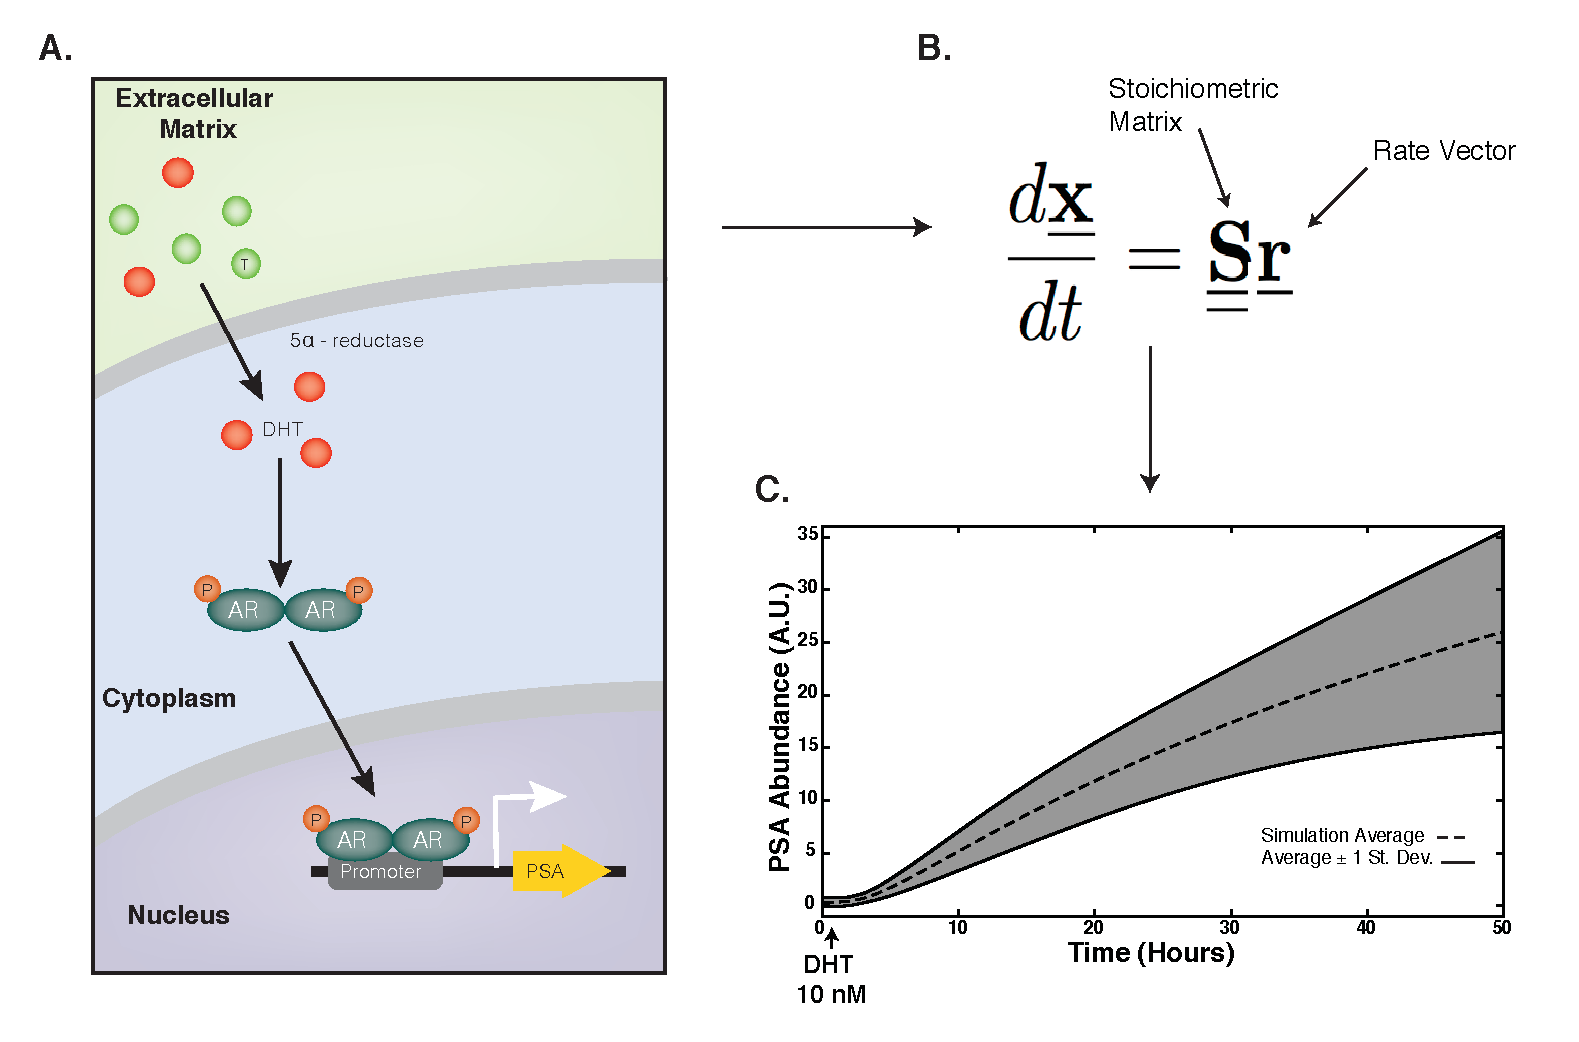
\includegraphics[width=1.0\textwidth]{./figs_chap1/Ode_Schematic.pdf}
\caption{Schematic of ODE analysis of the androgen receptor (AR) pathway. $\bf{A.}$ Simplified AR signal transduction network. $\bf{B.}$ The rate of change of network species x, dx/dt, is calculated from the stoichiometric matrix, $\mathbf{S}$, and the rate vector, $\mathbf{r}$. The stoichiometric matrix is formulated from the network shown in A. $\bf{C.}$ Continuos protein trajectory of PSA after addition of DHT.}
\label{fg:ODE_Model}
\end{figure}

\clearpage

\begin{figure}\centering
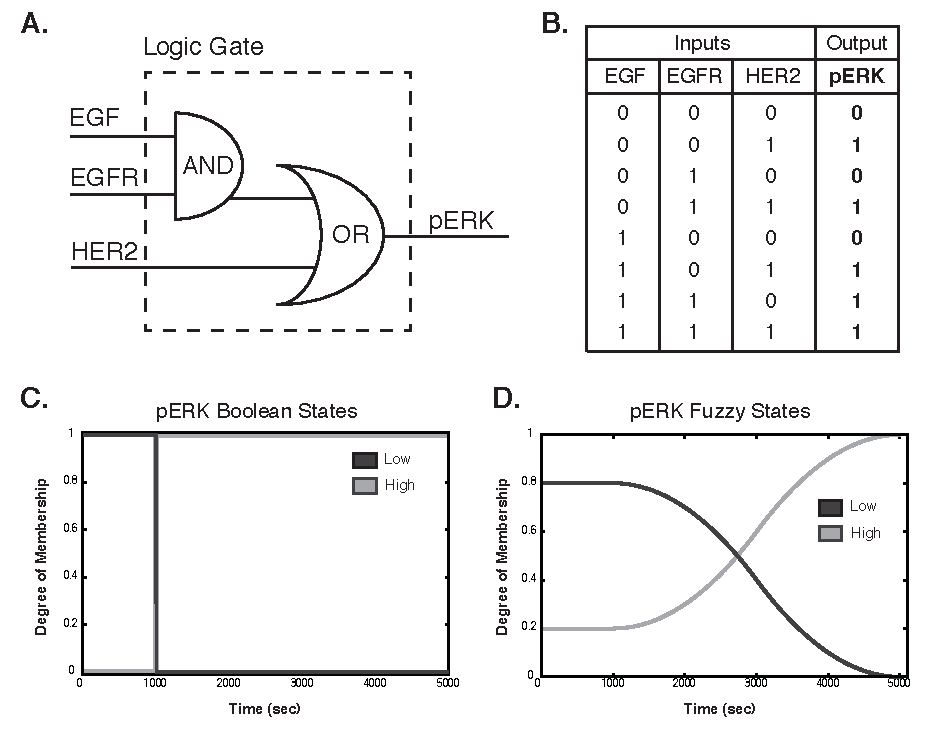
\includegraphics[width=1.0\textwidth]{./figs_chap1/Logic_Figure.pdf}
\caption{Schematic of a logical model framework. $\bf{A.}$ Simple logical model example based on EGFR and HER2 signaling. $\bf{B.}$ Boolean network truth table of the network in A. A value of zero denotes no expression and one denotes high expression, with pERK expression as the output. $\bf{C.}$, $\bf{D.}$ Boolean and fuzzy logic states of pERK, respectively. In the boolean model pERK can either be 1 or 0, while fuzzy logic allows for members to be in multiple groups.}
\label{fg:Logic_Model}
\end{figure}

\clearpage


%\end{comment}


\end{document}
